\documentclass[a4paper]{letter}
\usepackage{wallpaper}
\usepackage{geometry}
\usepackage{xcolor}
\usepackage[T1]{fontenc}
\usepackage[scaled]{helvet}
\usepackage{fontawesome5}
\usepackage[hidelinks]{hyperref}
\usepackage[french]{babel}
\usepackage{graphicx}
\usepackage{tikz}
\usepackage{setspace}
\usetikzlibrary{calc}

\renewcommand{\familydefault}{\sfdefault}

\geometry{
  a4paper,
  left=20pt,
  right=20pt,
  top=0pt,
  bottom=0pt,
  nohead,
  nofoot,
  nomarginpar
}

\ThisCenterWallPaper{1.1}{cvbg.png}
\newcommand{\skillsbar}[2]{%
  \begin{tikzpicture}
    \fill[gray!30] (0,0) rectangle (3,0.3);
    \fill[cyan] (0,0) rectangle (#2*3/100,0.3);
  \end{tikzpicture} \small #1
}
% Custom command for dividers
\newcommand{\divider}{\rule{\linewidth}{0.9pt}}

% ============================================================
% ======================== Left Side =========================
% ============================================================


\begin{document}
%\small
\begin{minipage}[t]{0.40\textwidth}
\setstretch{1.4} 
\setlength{\baselineskip}{1.2\baselineskip}
\color{white}
\vspace{5mm}

% ========================== Photo ============================

\begin{tikzpicture}
    \clip (0,0) circle (2cm);
    \node[anchor=center] at (0,0) {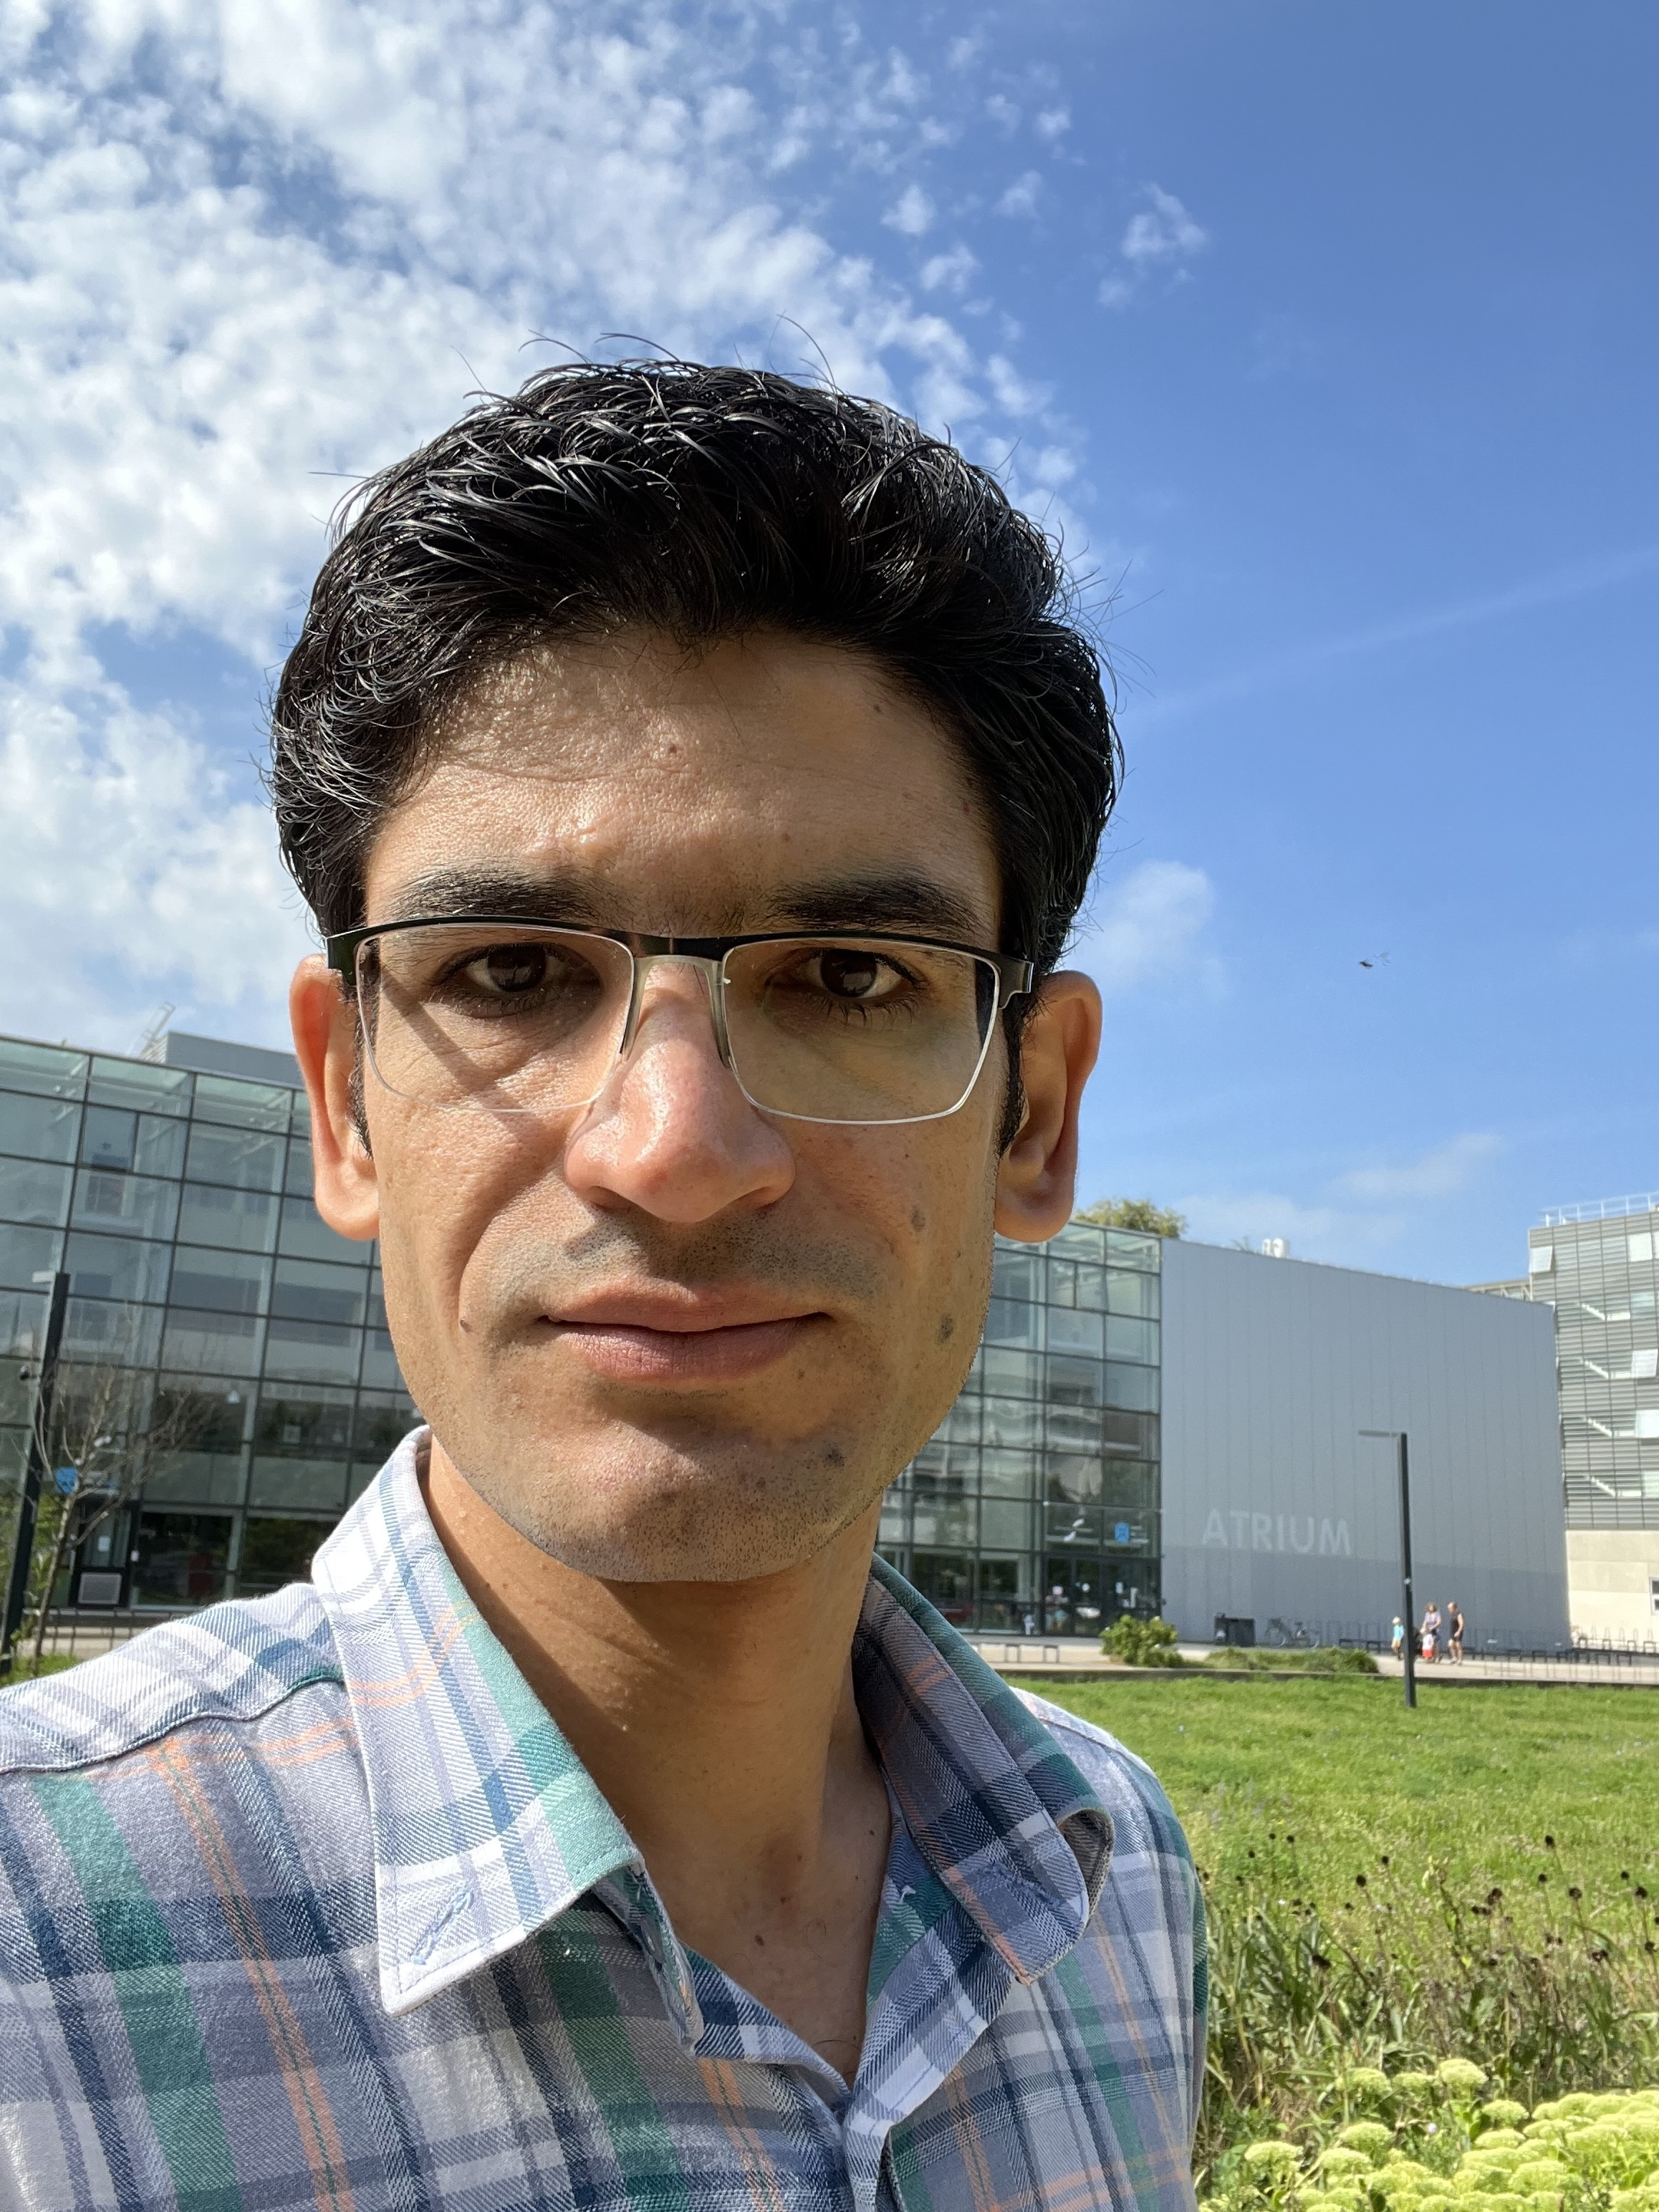
\includegraphics[width=4cm]{profile.jpg}};
\end{tikzpicture}

\vspace{5mm}

\divider

% ========================= Contact ===========================

\faPhone \quad 06 52 22 49 24

\faEnvelope \quad jafarizadeh89@gmail.com

\faGithub \quad \href{https://github.com/jafarizadeh}{jafarizadeh}

\faLinkedin \quad \href{https://www.linkedin.com/in/jafarizadeh/}{linkedin.com/in/jafarizadeh/}


\divider

% ================ Langage de Programmation ================
%\vspace{2mm}
{\large \textbf{Langues}}

\skillsbar{Persan (langue maternelle)}{100}

\skillsbar{Français}{75}

\skillsbar{Anglais}{50}

\divider
% ================ Langage de Programmation ================

{\large \textbf{Langage de Programmation}}

\faCircleNotch \quad Python

\faCircleNotch \quad C

\faCircleNotch \quad Swift

\faCircleNotch \quad HTML / CSS

\faCircleNotch \quad JavaScript

\faCircleNotch \quad SQL

\divider

% ===================== Logiciel de CAO ======================

{\large \textbf{Logiciel de CAO}}

\faCircleNotch \quad AutoCAD

\faCircleNotch \quad CATIA

\divider

% ========================== Réseau ==========================


{\large \textbf{Réseau}}

\faNetworkWired \quad CCNA

\faNetworkWired \quad CCNP (ENATSI)

\faNetworkWired \quad Fiber Optics

\end{minipage}
\hfill
\begin{minipage}[t]{0.60\textwidth}

% ============================================================
% ======================= Right  Side ========================
% ============================================================

\setlength{\baselineskip}{1.5\baselineskip}
\vspace{0.7cm}

{\huge Mehdi JAFARIZADEH}

\vspace{1cm}

% ========================= Éducation =========================

{\large \textbf{Éducation}}
\divider


{\textbf{Licence en Informatique}}

{\footnotesize Septembre 2021 - Présent}

{\textit{Université de Strasbourg, Strasbourg}}

\vspace{1mm}

\begin{itemize}
    \footnotesize
    
    \item Spécialisation en développement logiciel et intelligence artificielle
    \item Projets réalisés :
        \begin{itemize}
            \item Application mobile de gestion de tâches
            \item Système de recommandation basé sur le machine learning
        \end{itemize}
    \item Compétences acquises : Programmation avancée, Analyse de données, Apprentissage automatique
\end{itemize}

\vspace{3mm}


{\textbf{Bachelor en Génie des Énergies (équivalent Licence)}}

{\footnotesize Septembre 2014 - Décembre 2018}

{\textit{Université technologique de Quchan, Mashhad, Iran}}

\vspace{1mm}

\begin{itemize}
    \footnotesize
    \item Cours principaux :
        \begin{itemize}
            \item Thermodynamique avancée
            \item Énergies renouvelables
            \item Gestion de projets énergétiques
        \end{itemize}
    \item Projet de fin d'études : \textit{Simulé la consommation énergétique des habitations}
    \item Compétences acquises : Modélisation énergétique, Optimisation de l'efficacité énergétique, Utilisation de logiciels spécialisés
\end{itemize}

\vspace{3mm}

{\textbf{Diplôme en Comptabilité (Bac+2)}}

{\footnotesize Septembre 2007 - Décembre 2010}

{\textit{Université Azad de Kerman, Kerman, Iran}}

\vspace{1mm}
\begin{itemize}


    \footnotesize
    
    \item Cours principaux :
        \begin{itemize}
            \item Comptabilité financière
            \item Fiscalité
            \item Audit interne
        \end{itemize}
    \item Compétences acquises : Analyse financière, Conformité réglementaire
\end{itemize}




\vspace{3mm}

% ================ Expérience Professionnelle =================

{\large \textbf{Expérience Professionnelle}}
\divider

{\textbf{Directeur de l'association d'ingénierie énergétique}}

{\footnotesize Septembre 2015-Décembre 2017}
\begin{itemize}
   \footnotesize \item \textit{Université technologique de Quchan, Mashhad}
   \newline
   Animé des cours pédagogiques et organisé des concours scientifiques au sein de l'Association d'ingénierie énergétique, pour promouvoir les énergies renouvelables et sensibiliser aux enjeux de l'efficacité énergétique.
\end{itemize}

\vspace{3mm}

{ \textbf{Assistant enseignant}}

{ \footnotesize Septembre 2014-Décembre 2017}
\begin{itemize}
    \footnotesize \item \textit{Université technologique de Quchan, Mashhad}
    \newline
    Assistant enseignant en Mathématiques 1, Mathématiques 2 et Conversion énergétique : soutien aux étudiants, explication des concepts clés et aide à la préparation des travaux dirigés et des examens.
\end{itemize}





\vspace{3mm}

% ================ Contributions Académiques ==================

{\large \textbf{Contributions Académiques}}
\divider
\vspace{4mm}
\begin{itemize}
    \footnotesize \item {\textbf{Co-auteur}, \textit{Guide d’audit énergétique pour les étudiants de l’Université de Quchan, avec Dr. Majid Mahdavian, Publié en 2019}}


\end{itemize}

\vspace{3mm}


% ================ Projet ==================

{\large \textbf{Projets}}
\divider
\vspace{4mm}
\begin{itemize}
    \footnotesize \item {\textbf{Graphe dual d’un maillage}, \textit{Développé en C un algorithme transformant un maillage en graphe dual et optimisé le tri des arêtes et la coloration avec Dijkstra.}}
    \vspace{2mm}
    \footnotesize \item {\textbf{web Programmation}, \textit{Conçu et développé un site portfolio en utilisant JavaScript et PHP, intégrant des fonctionnalités interactives et dynamiques.}}
    \vspace{2mm}
    \footnotesize \item {\textbf{EES}, \textit{Simulé et analysé une centrale électrique avec le logiciel EES, optimisant les performances énergétiques.}}


\end{itemize}

\vspace{3mm}

% ================ Formations Complémentaires ==================

%{\large \textbf{Formations Complémentaires}}
%\divider
%\vspace{4mm}
%\begin{itemize}
    
    %\footnotesize \item {\textbf{CCNP ENARSI 300-410}, \textit{Formation CCNP ENARSI 300-410 : maîtrise avancée du routage et des services d'infrastructure réseau pour les environnements complexes.}}
    %\vspace{2mm}
    %\footnotesize \item {\textbf{CCNA 200-301}, \textit{Formation CCNA 200-301 : compétences fondamentales en réseaux, incluant la configuration, gestion et dépannage d'infrastructures réseaux.}}
    %\vspace{2mm}
    %\footnotesize \item {\textbf{Wireshark for Beginners: Capture Packets}, \textit{Formation Wireshark for Beginners : initiation à la capture et l'analyse de paquets réseau pour le diagnostic et le dépannage.}}
    %\vspace{2mm}
    %\footnotesize \item {\textbf{Initiation à Wireshark pour l’analyse de paquets sous linux}, \textit{Initiation à Wireshark : capture et analyse de paquets réseau sous Linux pour le diagnostic et la sécurité.}}
    %\vspace{2mm}
    %\footnotesize \item {\textbf{Configure VLANs on Cisco Switches}, \textit{Configuration de VLANs sur des commutateurs Cisco pour segmenter et sécuriser les réseaux.}}
    %\vspace{2mm}
    %\footnotesize \item {\textbf{Google Cloud Fundamentals: Core Infrastructure}, \textit{Formation Google Cloud Fundamentals : maîtrise des concepts clés de l'infrastructure cloud, y compris les services de calcul, de stockage et de gestion de réseau.}}
    

%\end{itemize}

%\vspace{3mm}


\end{minipage}

% ========================== Code QR ==========================

\begin{tikzpicture}[remember picture,overlay]
    \node[anchor=south east,inner sep=0pt] at ($(current page.south west)+(6.5cm,+2.5cm)$) {
        
\includegraphics[width=2cm]{Documentation_FR.png}
    };
    
    \node[anchor=south east,inner sep=0pt] at ($(current page.south west)+(4cm,+2.5cm)$) {
        \begin{minipage}[t]{3.05cm} 
            \color{white} \scriptsize \href{https://drive.google.com/file/d/1jKjZWYadaikaPetkEmjoupWWh_w1sMKA/view?usp=drive_link}{Veuillez cliquer ici ou scanner ce code QR pour accéder à un dossier détaillé de mes contributions académiques et professionnelles.}
        \end{minipage}
    };


    \node[anchor=south west,inner sep=0pt] at ($(current page.south west)+(0.8cm,1cm)$) {
        \begin{minipage}[t]{4cm}
            \tiny \textcolor{white}{Dernière mise à jour: \today}
        \end{minipage}
    };
\end{tikzpicture}

\end{document}
